\section{Early investigations on visual quality in more complex environments}
\label{app:additonal_experiments}

In the main body of the paper, we evaluated the utility of \textsc{diamond} for the purpose of training RL agents in a world model on the well-established Atari 100k benchmark \citep{kaiser2019atari100k}, and demonstrated \textsc{diamond}'s diffusion world model could be applied to model a more complex 3D environment from the game \textit{Counter-Strike: Global Offensive}. In this section, we provide early experiments investigating the effectiveness of \textsc{diamond}'s diffusion world model by directly evaluating the visual quality of the trajectories they generate. The two environments we consider are presented in Section \ref{app:subsec:environments} below.

\subsection{Environments}
\label{app:subsec:environments}

\textbf{CS:GO.} 
We use the \textit{Counter-Strike: Global Offensive} dataset introduced by \citet{pearce2022counter}. Here we use the \textit{Clean} dataset containing 190k frames (3.3 hours) of high-skill human gameplay, captured on the \textit{Dust II} map. This contains observations and actions (mouse and keyboard) captured at 16Hz. We use 150k frames (2.6 hours) for training and 40k frames (0.7 hours) for evaluation. We resize observations to 64$\times$64 pixels, and use no augmentation.
%\footnote{\href{https://github.com/TeaPearce/Counter-Strike_Behavioural_Cloning}{\texttt{https://github.com/TeaPearce/Counter\-Strike\_Behavioural\_Cloning}}}.

\textbf{Motorway driving.} We use the dataset from \citet{santana2016learning}\footnote{\href{https://github.com/commaai/research}{\texttt{https://github.com/commaai/research}}}, which contains camera and metadata captured from human drivers on US motorways. We select only trajectories captured in daylight, and exclude the first and last 5 minutes of each trajectory (typically traveling to/from a motorway), leaving 4.4 hours of data. We use five trajectories for training (3.6 hours) and two for testing (0.8 hours). We downsample the dataset to 10Hz, resize observations to 64$\times$64, and for actions use the (normalized) steering angle and acceleration. During training, we apply data augmentation of shift \& scale, contrast, brightness, and saturation, and mirroring.

We note that the purpose of our investigation is to train and evaluate \textsc{diamond}'s diffusion model on these static datasets, and that we do not perform reinforcement learning, since there is no standard reinforcement learning protocol for these environments.


\subsection{Diffusion Model Architectures}

We consider two potential diffusion model architectures, summarized in Figure \ref{fig_architectures}.

\begin{figure}[h]
    \begin{center}
    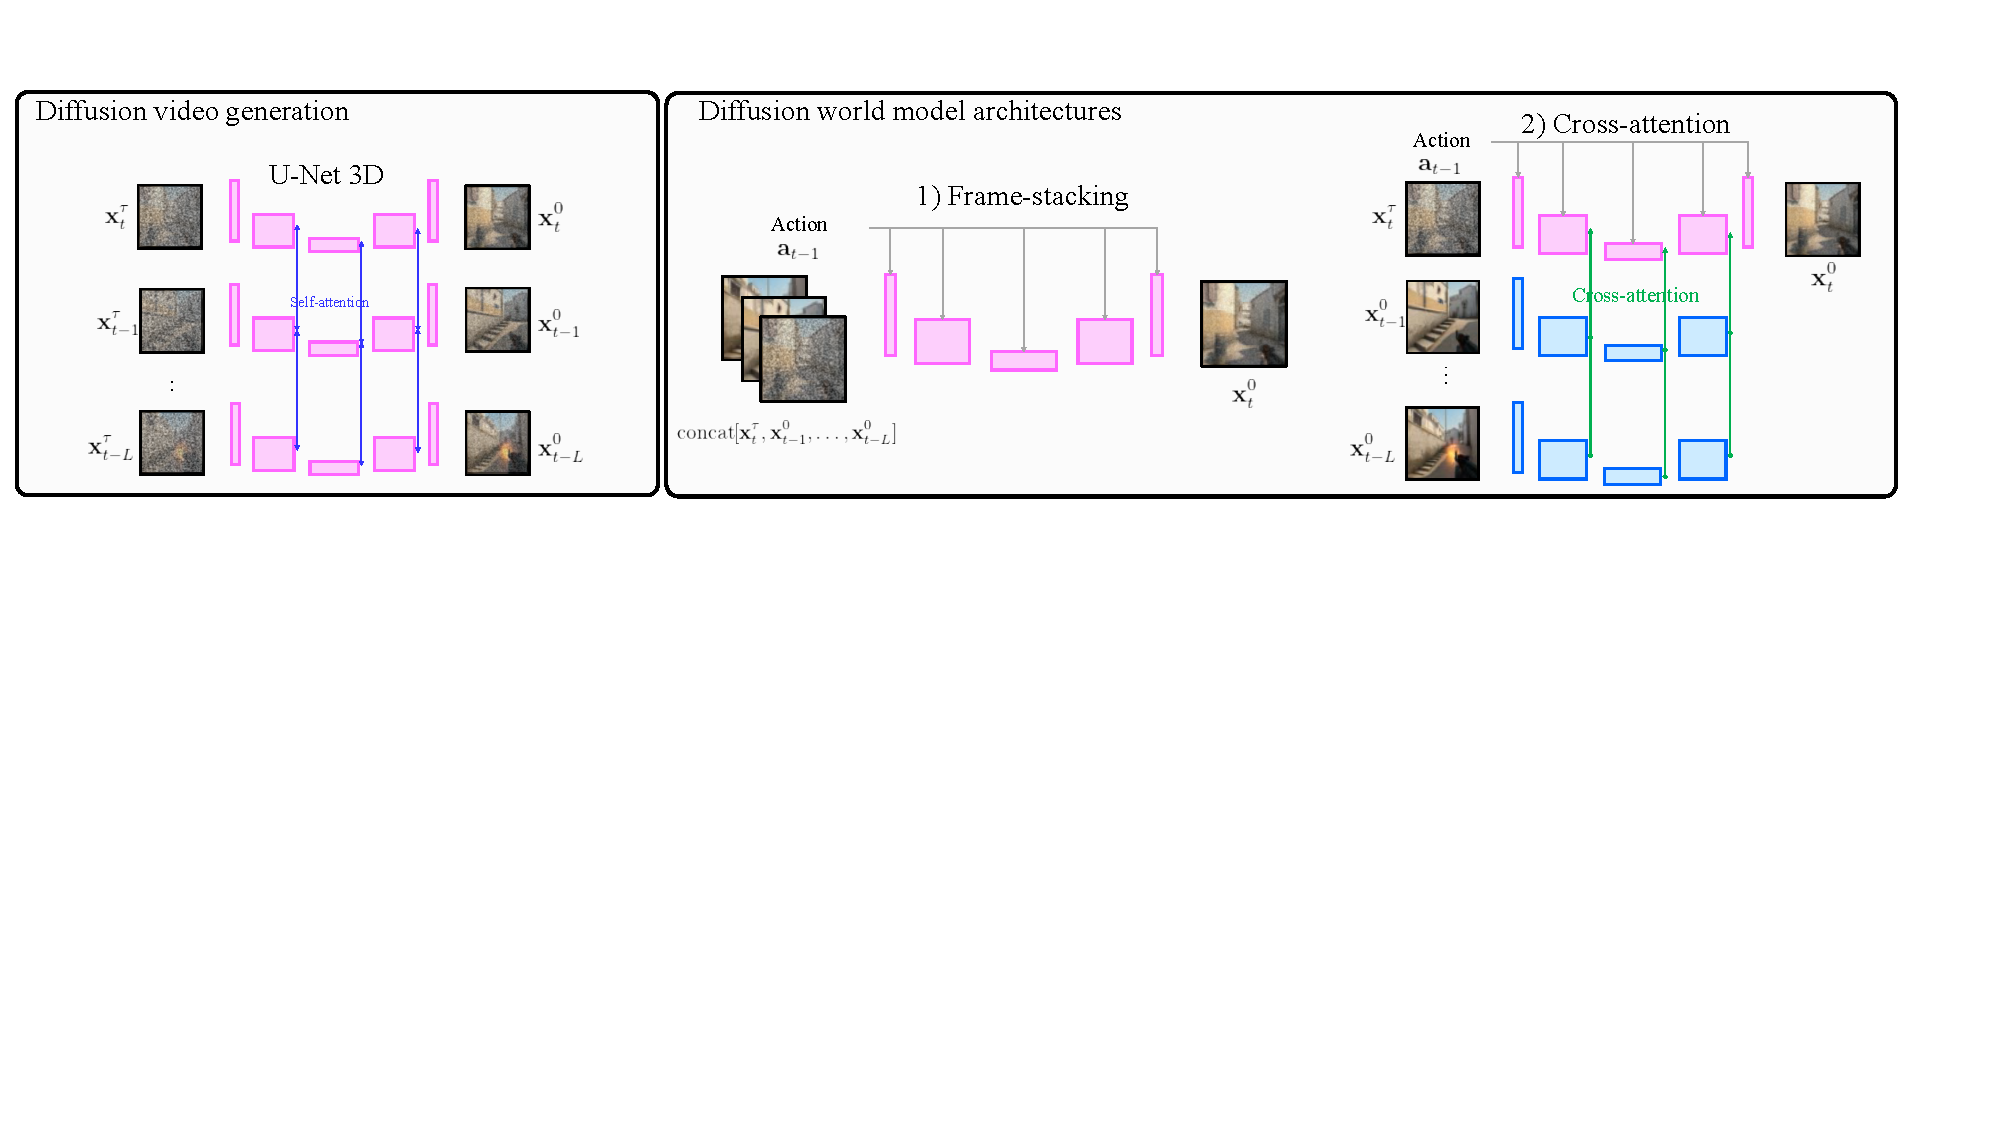
\includegraphics[width=0.99\columnwidth]{images/architectures_02.pdf}
    % \vskip -0.18in
    \caption{We tested two architectures for \textsc{diamond}'s diffusion model which condition on previous image observations in different ways. To illustrate differences with typical video generation models, we also visualize a U-Net 3D \citep{unet3d} which diffuses a block of frames simultaneously.}
    \label{fig_architectures}
    \end{center}
\end{figure}

\textbf{Frame-stacking.} The simplest way to condition on previous observations is by concatenating the previous $L$ frames together with the next noised frame, $\operatorname{concat}[ \x_t^{\tau}, \x_{t-1}^0, \dots, \x_{t-L}^0]$, which is compatible with a standard U-Net 2D \citep{ronneberger2015unet}.
This architecture is particularly attractive due to its lightweight construction, requiring minimal additional parameters and compute compared to typical image diffusion. This is the architecture we used for the main body of the paper.
% Experiments in Section \ref{sec_experiments} show this to be a surprisingly powerful mechanism for modeling both simple and complex environments. 

\textbf{Cross-attention.} 
The U-Net 3D \citep{unet3d}, also displayed for comparison in Figure \ref{fig_architectures}, is a leading architecture in video diffusion \citep{ho2022video}. We adapted this design to have an autoregressive cross-attention architecture, formed of a core U-Net 2D, that only receives a single noised frame as direct input, but which cross-attends to the activations of a separate history encoder network. This encoder is a lightweight version of the U-Net 2D architecture. Parameters are shared for all $L$ encoders, and each receives the relative environment timestep embedding as input.
The final design differs from the U-Net 3D which diffuses all frames jointly, shares parameters across networks, and uses self-, rather than cross-, attention.

\subsection{Metrics, Baselines and Compute}
\textbf{Metrics.}
To evaluate the visual quality of generated trajectories, we use the standard Fréchet Video Distance (\textbf{FVD}) \citep{unterthiner2018towards} as implemented by \citet{skorokhodov2022stylegan}. This is computed between 1024 real videos (taken from the test set), and 1024 generated videos, each 16 frames long (1-2 seconds). Models condition on $L=6$ previous real frames, and the real action sequence. On this same data, we also report the Fréchet Inception Distance (\textbf{FID}) \citep{heusel2017gans}, which measures the visual quality of individual observations, ignoring the temporal dimension. For these same sets of videos, we also compute the \textbf{LPIPS} loss \citep{zhang2018lpips} between each \textit{pair} of real/generated observations \citep{yan2023teco}.
\textbf{Sampling rate} describes the number of observations that can be generated, in sequence, by a single Nvidia RTX A6000 GPU, per second.

\textbf{Baselines.}
We compare against two well-established world model methods; DreamerV3 \citep{hafner2023dreamerv3} and \textsc{iris} \citep{iris2023}, adapting the original implementations to train on a static dataset. We ensured baselines used a similar number of parameters to \textsc{diamond}. Two variants of \textsc{iris} are reported; image observations are discretized into $K=16$ tokens (as used in the original work), or into $K=64$ tokens (achieved with one less down/up-sampling layer in the autoencoder, see Appendix E of \citet{iris2023}), which provide the potential for modeling higher-fidelity visuals. 
% The full list of hyperparameters is provided in the Appendix.
% IRIS: 35M for autoencoder, 88M for transformer, seq length 8...


\textbf{Compute.}
All models (baselines and \textsc{diamond}) were trained for 120k updates with a batch size of 64, on up to 4$\times$A6000 GPUs. Each training run took between 1-2 days.

\subsection{Analysis}

\begin{table}[h]
\caption{Results for 3D environments. These metrics compare observations from real trajectories and generated trajectories. The generated trajectories are conditioned on an initial set of $L=6$ observations and a real sequence of actions.}
\label{tab:video_results}
\begin{center}
\resizebox{0.999 \columnwidth}{!}{
\begin{tabular}{ l c c c c c c c c}
\toprule
\multicolumn{1}{c}{}  & \multicolumn{3}{c}{ ------------ \textbf{CS:GO} ------------} & \multicolumn{3}{c}{ ----------- \textbf{Driving} ----------- } & \multicolumn{1}{c}{\bf Sample rate} & \multicolumn{1}{c}{\bf Parameters} \\
\multicolumn{1}{l}{\bf Method}  & \multicolumn{1}{c}{\bf FID $\downarrow$} & \multicolumn{1}{c}{\bf FVD $\downarrow$ } & \multicolumn{1}{c}{\bf LPIPS $\downarrow$ } & \multicolumn{1}{c}{\bf FID $\downarrow$} & \multicolumn{1}{c}{\bf FVD $\downarrow$} & \multicolumn{1}{c}{\bf LPIPS $\downarrow$ }  & \multicolumn{1}{c}{\bf (Hz) $\uparrow$} & \multicolumn{1}{c}{\bf (\#)} \\ 
\hline \\
DreamerV3 & 106.8 & 509.1 & 0.173 & 167.5 & 733.7 & 0.160 & 266.7 & 181M \\
IRIS ($K=16$) & 24.5 & 110.1 & 0.129 & 51.4 & 368.7 & 0.188 & 4.2 & 123M \\
IRIS ($K=64$) & 22.8 & 85.7 & 0.116 & 44.3 & 276.9 & 0.148 & 1.5 & 111M \\
$\textsc{diamond}$ frame-stack (ours) & 9.6 & 34.8 & 0.107 & 16.7 & 80.3 & 0.058 & 7.4 & 122M \\
$\textsc{diamond}$ cross-attention (ours) & 11.6 & 81.4 & 0.125 & 35.2 & 299.9 & 0.119 & 2.5 & 184M \\
\bottomrule
\end{tabular}
}
\end{center}
\end{table}


Table \ref{tab:video_results} reports metrics on the visual quality of generated trajectories, along with sampling rates and number of parameters, for the frame-stack and cross-attention \textsc{diamond} architectures, compared to baseline methods. 
\textsc{diamond} outperforms the baselines across all visual quality metrics. 
This validates the results seen in the wider video generation literature, where diffusion models currently lead, as discussed in Section \ref{sec:related_work}.
The simpler frame-stacking architecture performs better than cross-attention, something surprising given the prevalence of cross-attention in the video generation literature. We believe the inductive bias provided by directly feeding in the input, frame-wise, may be well suited to autoregressive generation. Overall, these results indicate \textsc{diamond} frame-stack $>$ \textsc{diamond} cross-attention $\approx$ IRIS 64 $>$ IRIS 16 $>$ DreamerV3, which we found corresponds to our intuition from visual inspection.

In terms of sampling rate, \textsc{diamond} frame-stack (with 20 denoising steps) is faster than \textsc{iris} ($K=16$). \textsc{iris} suffers from a further 2.8$\times$ slow down for the $K=64$ version, verifying its sample time is bottlenecked by the number of tokens $K$.
On the other hand, DreamerV3 is an order of magnitude faster -- this derives from its independent, rather than joint, sampling procedure, and the flip-side of this is the low visual quality of its trajectories. 

\newpage


Figure \ref{fig_generation_egs} below shows selected examples of the trajectories produced by \textsc{diamond} in CS:GO and motorway driving.
% Trajectories produced by baselines are given in Appendix \tp{x}.
% , and comparisons with baselines in Appendix Figures \tp{x} \& \tp{y}.
The trajectories are plausible, often even at time horizons of reasonable length. In CS:GO, the model accurately generates the correct geometry of the level as it passes through the doorway into a new area of the map. In motorway driving, a car is plausibly imagined overtaking on the left.

\begin{figure}[h!]
    \begin{center}
    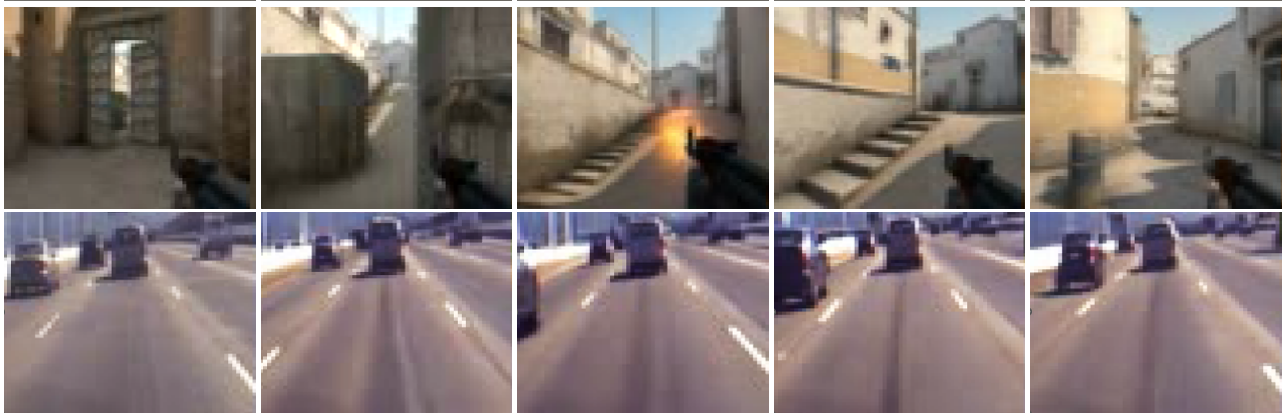
\includegraphics[width=0.8\columnwidth, height=0.4\columnwidth]{images/generation_egs_02.png}
    % \vskip -0.18in
    \caption{Example trajectories sampled every 25 timesteps from \textsc{diamond} (frame stack) for the modern 3D first-person shooter CS:GO (top row), and real-world motorway driving (bottom row).}
    \label{fig_generation_egs}
    \end{center}
\end{figure}


While the above experiments use real sequences of actions from the dataset, we also investigated how robust $\textsc{diamond}$ (frame stack) was to novel, user-input actions.
Figure \ref{fig_driving_action} shows the effect of the actions in motorway driving -- conditioned on the same $L=6$ real frames, we generate trajectories conditioned on five different action sequences. In general the effects are as intended, e.g. steer straight/left/right moves the camera as expected.
Interestingly, when `slow down' is input, the distance to the car in front decreases since the model predicts that the traffic ahead has come to a standstill.
%This is an interesting causal confusion, since from the action alone, slowing down should in principle \textit{increase} the distance to the car in front. 
Figure \ref{fig_csgo_action} shows similar sequences for CS:GO. For the common actions (mouse movements and fire), the effects are as expected, though they are unstable beyond a few frames, since such a sequence of actions is unlikely to have been seen in the demonstration dataset.
% We found that $\textsc{wm}$ had not learned to model the impact of less common actions such as `jump'.
We note that these issues -- the causal confusion and instabilities -- are a symptom of training world models on offline data, rather than being an inherent weakness of $\textsc{diamond}$.
% Also acknowledge the offdistribution problem, but more a problem of data than model.


\begin{figure}[h!]
    \begin{center}
    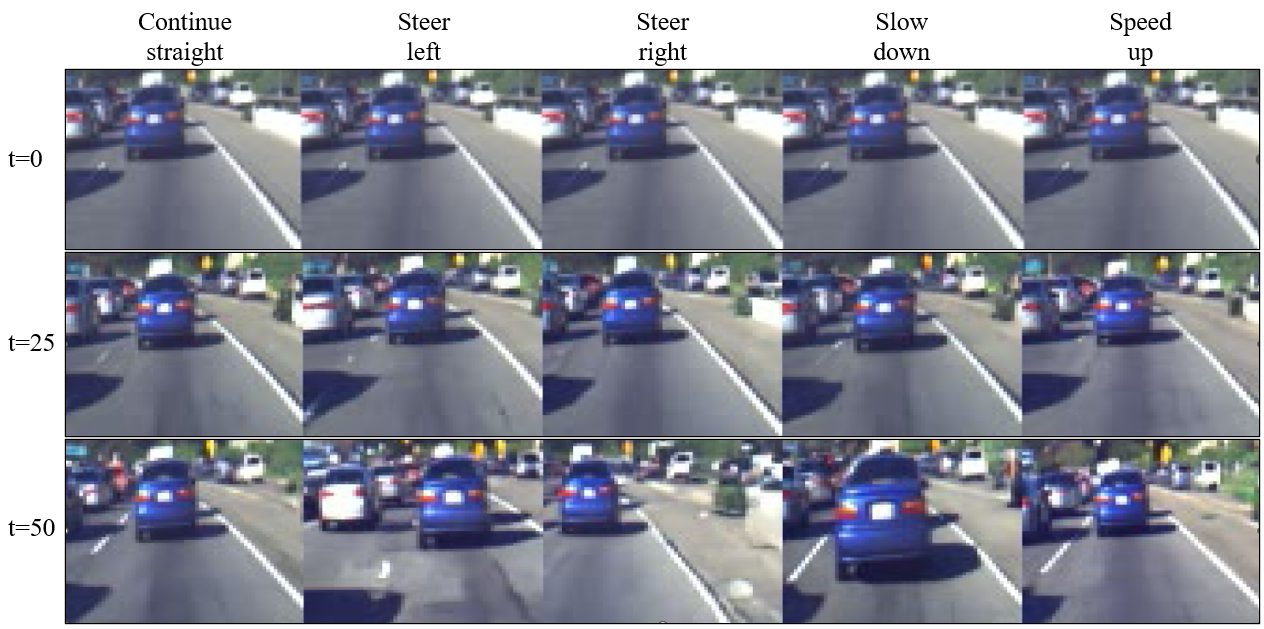
\includegraphics[width=0.99\columnwidth]{images/driving_action_02.png}
    % \vskip -0.18in
    \caption{Effect of fixed actions on sampled trajectories in motorway driving. Conditioned on the same initial observations, we rollout the model applying differing actions. Interestingly, the model has learnt to associate 'Slow down' and 'Speed up' actions to the whole traffic slowing down and speeding up.}
    \label{fig_driving_action}
    \end{center}
\end{figure}


\begin{figure}[t!]
    \begin{center}
    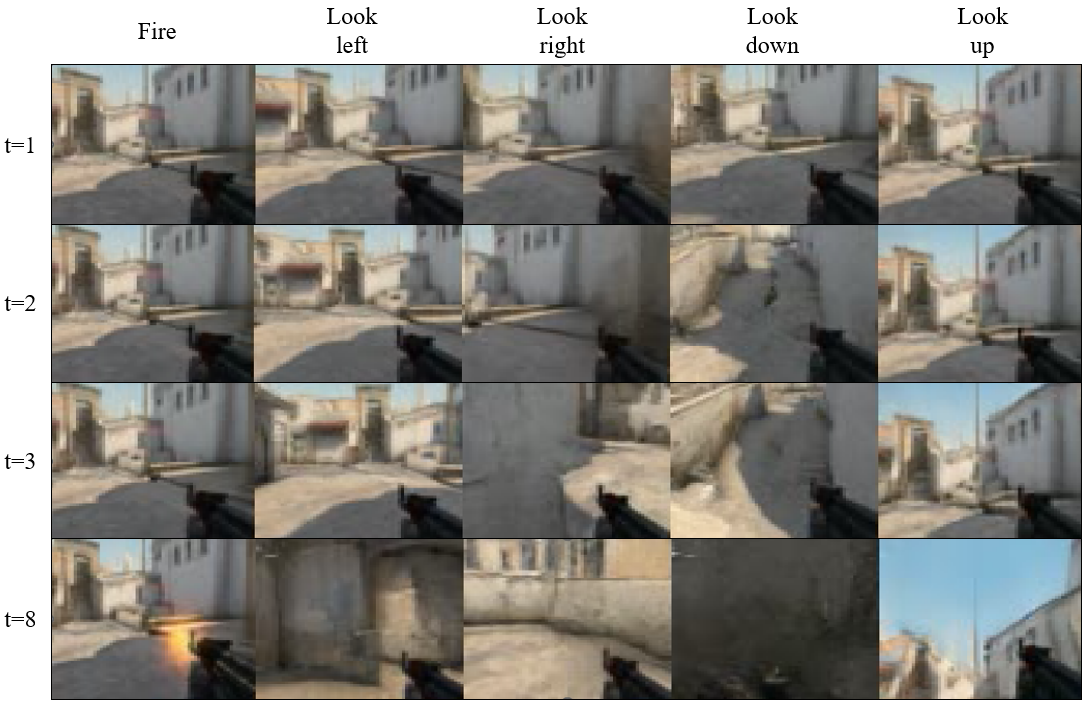
\includegraphics[width=0.9\columnwidth]{images/csgo_action_01.png}
    % \vskip -0.18in
    \caption{Effect of fixed actions on sampled trajectories in CS:GO. Conditioned on the same initial observation, we rollout the model applying differing actions. Whilst in immediate frames these have the intended effect, for longer roll-outs the observations can degenerate. For instance, it would have been very unlikely for the human demonstrator to look directly into ground in this game state, so the world model is unable to generate a plausible trajectory here, and instead snaps onto another area of the map when looking down does make sense.}
    \label{fig_csgo_action}
    \end{center}
\end{figure}
\clearpage